\documentclass{article}

\usepackage[T1]{fontenc}
\usepackage[utf8]{inputenc}
\usepackage{times}

\usepackage[font=small,labelfont=bf,tableposition=top]{caption}
\usepackage{graphicx}
\usepackage{natbib} 

\usepackage{amsmath}
\usepackage{amsfonts}
\usepackage{amssymb}
\usepackage{color, soul}
\usepackage{hyperref}
\usepackage{algorithmicx}
\usepackage{algpseudocode}
\usepackage{subfigure}
\usepackage{stmaryrd}

\renewcommand{\vec}[1]{\boldsymbol{{#1}}} 
\newcommand{\duesoon}[1]{{\sethlcolor{green}\hl{#1}}}
\usepackage{mathrsfs}


\newtheorem{theorem}{Theorem}
\newtheorem{acknowledgement}[theorem]{Acknowledgement}
\newtheorem{algorithm}[theorem]{Algorithm}
\newtheorem{axiom}[theorem]{Axiom}
\newtheorem{case}[theorem]{Case}
\newtheorem{claim}[theorem]{Claim}
\newtheorem{conclusion}[theorem]{Conclusion}
\newtheorem{condition}[theorem]{Condition}
\newtheorem{conjecture}[theorem]{Conjecture}
\newtheorem{corollary}[theorem]{Corollary}
\newtheorem{criterion}[theorem]{Criterion}
\newtheorem{definition}[theorem]{Definition}
\newtheorem{example}[theorem]{Example}
\newtheorem{exercise}[theorem]{Exercise}
\newtheorem{lemma}[theorem]{Lemma}
\newtheorem{notation}[theorem]{Notation}
\newtheorem{problem}[theorem]{Problem}
\newtheorem{proposition}[theorem]{Proposition}
\newtheorem{remark}[theorem]{Remark}
\newtheorem{solution}[theorem]{Solution}
\newtheorem{summary}[theorem]{Summary}
\newenvironment{proof}[1][Proof]{\textbf{#1.} }{\ \rule{0.5em}{0.5em}}

\newtheorem{guess}{Definition}
\newcommand{\comment}[1] {}
\newcommand{\Norder} {N}
\newcommand{\order}{\mathcal{O}}
\newcommand{\Npoints} {N_p}
\newcommand{\Nfaces} {N_{f}}
\newcommand{\Nelements} {N_e}

\newcommand{\eps}{\varepsilon}
\newcommand{\Dweak}{\wt{D}}
\newcommand{\diff}[2] {\frac{\partial #1}{\partial #2}}
\newcommand{\dxx}[2] {\frac{\partial^2 #1}{\partial {#2}^2}}
\newcommand{\difft}[2] {\frac{d #1}{d #2}}
\newcommand{\dxxt}[2] {\frac{d^2 #1}{d {#2}^2}}
\newcommand{\lagrange}[1] {\frac{d #1}{dt}}
\newcommand{\lebesgue}{\parallel I \parallel}
\newcommand{\polysp}{\mathcal{P}_N}
\newcommand{\laplacian}{\nabla^2}
\newcommand{\divergence}{\nabla \cdot}
\newcommand{\inte}{\int_{\mbox{\footnotesize ${\Omega_e}$}}}
\newcommand{\intb}{\int_{\mbox{\footnotesize ${\Gamma_e}$}}}
\newcommand{\intce}{\int_{\mbox{\footnotesize ${\widehat{\Omega}_e}$}}}
\newcommand{\intcb}{\int_{\mbox{\footnotesize ${\widehat{\Gamma}_e}$}}}
\newcommand{\intg}{\int_{\mbox{\footnotesize ${\Omega}$}}}
\newcommand{\intgb}{\int_{\mbox{\footnotesize ${\Gamma}$}}}
\newcommand{\intv}{\int_{\mbox{\footnotesize ${\sigma}$}}}
\newcommand{\sumv}{\sum_{K=1}^{N_{\mathrm{lev}}}}
\newcommand{\sumk}{\sum_{L=1}^{K}}
\newcommand{\sumN}{\sum_{i=1}^{N+1}}
\newcommand{\half}{\frac{1}{2}}
\newcommand{\inti}{\int_{\mbox{\footnotesize\sf I}}}
\newcommand{\intbd}{\oint_{\mbox{\footnotesize ${\delta}$\sf D}}}
\newcommand{\intbi}{\oint_{\mbox{\footnotesize ${\delta}$\sf I}}}
\newcommand{\ldnorm}[1]{\left\| #1 \right\|_{\mbox{\footnotesize \sf D}} }
\newcommand{\lonorm}[1]{\left\| #1 \right\|_{\Omega}}
\newcommand{\spc}[1]{\mbox{\sf #1}}
\newcommand{\ope}[1]{{\cal #1}}
\newcommand{\mt}[1]{{\rm #1}}
\newcommand{\dis}{\displaystyle}
\newcommand{\ve}{\varepsilon}
\newcommand{\ov}{\overline}
\newcommand{\wt}{\widetilde}
\newcommand{\wh}{\widehat}
\newcommand{\Dhat}{\widehat{D}}
\newcommand{\be}{\begin{equation}}
\newcommand{\ee}{\end{equation}}
\newcommand{\bea}{\begin{eqnarray*}}
\newcommand{\eea}{\end{eqnarray*}}
\newcommand{\Jace}{J^{(e)}}
\newcommand{\Jacl}{J^{(l)}}
\def\bepsilon{\mbox{\boldmath $\epsilon $}}
\def\bpsi{\mbox{\boldmath $\psi $}}
\def\bphi{\mbox{\boldmath $\phi $}}
\def\bmu{\mbox{\boldmath $\mu $}}
\def\Et{ \tilde{E} }
\def\Ht{ \tilde{H} }
\def\sdot{ \dot{\sigma} }

\newcommand{\fstar}{f^{(*)}}

\DeclareMathOperator{\Span}{span}
\DeclareMathOperator{\Dim}{dim}

\newcommand{\polyquad}{\mathcal{Q}_{N}}
\newcommand{\polyP}{\mathcal{P}_{N}}
\newcommand{\polyPnpm}{\mathcal{P}_{(N+M)}}
\newcommand{\polyPd}{\mathcal{P}_{d}}
\newcommand{\polyPnm}{\mathcal{P}_{N,M}}
\newcommand{\polyPn}{\mathcal{P}_{N,0}}
\newcommand{\transpose}{^{\mathcal{T}}}

\newcommand{\vecQ}{\vec{Q}}
\newcommand{\vecQe}{\vec{Q}^{(e)}}
\newcommand{\vecFe}{\vec{\mathcal{F}}^{(e)}}
\newcommand{\statevec}{\vec{Y}}
\newcommand{\statevecN}{\vec{Y}_N^{(e)}}
\newcommand{\statestage}{\vec{\mathcal{Y}}}
\newcommand{\Ftensor}{\vec{F}(\qvector)}
\newcommand{\FtensorN}{\vec{F}\left( \qvectorN \right)}
\newcommand{\FtensorStar}{\vec{F}\left( \qvector_N^{(e,k)} \right)}
\newcommand{\Svector}{S(\qvector)}
\newcommand{\SvectorN}{S \left( \qvectorN \right)}
\newcommand{\qref}{\vec{q}_0}
\newcommand{\qvectorb}{\vec{q}_b}
\newcommand{\qtt}{\vec{q}_{tt}}
\newcommand{\qhat}{\widehat{\vec{q}}}
\newcommand{\qhatb}{\widehat{\vec{q}}_b}
\newcommand{\qelem}{q^{(e)}}
\newcommand{\rhoref}{\rho_0}
\newcommand{\piref}{\pi_0}
\newcommand{\Thetaref}{\Theta_0}
\newcommand{\Gref}{G_0}
\newcommand{\Tref}{T_0}
\newcommand{\thetaref}{\theta_0}
\newcommand{\Pref}{{P}_0}
\newcommand{\Eref}{{E}_0}
\newcommand{\Href}{{h}_0}
\newcommand{\rhohat}{\widehat{\rho}}
\newcommand{\pihat}{\widehat{\pi}}
\newcommand{\Phat}{\widehat{P}}
\newcommand{\uvechat}{\widehat{{\mbox{\boldmath$u$\unboldmath}}}}
\newcommand{\uhathat}{\widehat{\widehat{{\mbox{\boldmath$u$\unboldmath}}}}}
\newcommand{\Uhat}{\widehat{{\mbox{\boldmath$U$\unboldmath}}}}
\newcommand{\Uhathat}{\widehat{\widehat{{\mbox{\boldmath$U$\unboldmath}}}}}
\newcommand{\thetahat}{\widehat{\theta}}
\newcommand{\Thetahat}{\widehat{\Theta}}
\newcommand{\Ehat}{\widehat{E}}
\newcommand{\uhat}{\widehat{u}}
\newcommand{\vhat}{\widehat{v}}
\newcommand{\what}{\widehat{w}}
\newcommand{\pitt}{\pi_{tt}}
\newcommand{\rhott}{\rho_{tt}}
\newcommand{\Ett}{E_{tt}}
\newcommand{\Utt}{\vec{U}_{tt}}
\newcommand{\uvectt}{\vec{u}_{tt}}
\newcommand{\utt}{u_{tt}}
\newcommand{\vtt}{v_{tt}}
\newcommand{\wtt}{w_{tt}}
\newcommand{\Ptt}{P_{tt}}
\newcommand{\vecPtt}{\vec{P}_{tt}}
\newcommand{\Thetatt}{\Theta_{tt}}
\newcommand{\thetatt}{\theta_{tt}}
%Projector Matrices
\newcommand{\projmatrix}{\vec{\mathcal{P}}}
\newcommand{\qmatrix}{\vec{\mathcal{Q}}}
\newcommand{\pcmatrix}{\vec{\mathcal{P}}_C}
\newcommand{\Cmatrix}{\left(\vec{\mathcal{C}}^{(e,f)}\right)\transpose}
\newcommand{\Dmatrix}{\vec{D}^{(e)}}
\newcommand{\Dwmatrix}{\wt{\vec{D}}^{(e)}}
\newcommand{\Mmatrix}{M^{(e)}}
\newcommand{\Fmatrix}{\vec{F}^{(e,l)}}
\newcommand{\Gmatrix}{\mathcal{G}}
\newcommand{\Umatrix}{\mathcal{U}^{(e,f)}}
\newcommand{\amatrix}{\vec{\mathcal{A}}}
\newcommand{\rmatrix}{\vec{\mathcal{R}}}
%Vectors
\newcommand{\nvector}{\wh{\vec{n}}_{\Gamma}}
\newcommand{\nhat}{\wh{\vec{n}}}
\newcommand{\ivector}{\wh{\vec{i}}}
\newcommand{\jvector}{\wh{\vec{j}}}
\newcommand{\kvector}{\wh{\vec{k}}}
\newcommand{\rvector}{\wh{\vec{r}}}
\newcommand{\svector}{\wh{\vec{s}}}
\newcommand{\tvector}{\wh{\vec{t}}}
\newcommand{\vvector}{\wh{\vec{v}}}
\newcommand{\Qvector}{\vec{Q}}
%Vectors
\newcommand{\ur}{{u}^{(r)}}
\newcommand{\us}{{u}^{(s)}}
\newcommand{\ut}{{u}^{(t)}}
\newcommand{\urtt}{{u}_{tt}^{(r)}}
\newcommand{\ustt}{{u}_{tt}^{(s)}}
\newcommand{\uttt}{{u}_{tt}^{(t)}}
\newcommand{\urhat}{\widehat{u}^{(r)}}
\newcommand{\ushat}{\widehat{u}^{(s)}}
\newcommand{\uthat}{\widehat{u}^{(t)}}
%Other Operators
\newcommand{\grad}{\vec{\nabla}}
\newcommand{\Grad}{\vec{\nabla}}
\newcommand{\Dskew}{\mathcal{D}}

\def\bepsilon{\mbox{\boldmath $\epsilon $}}
\def\bpsi{\mbox{\boldmath $\psi $}}
\def\bphi{\mbox{\boldmath $\phi $}}
\def\bmu{\mbox{\boldmath $\mu $}}
\def\Et{ \tilde{E} }
\def\Ht{ \tilde{H} }
\def\sdot{ \dot{\sigma} }
%\renewcommand{\thetable}{\Roman{table}}
%\renewcommand{\thefigure}{\arabic{figure}}

%\DeclareMathOperator{\Span}{span}
%\DeclareMathOperator{\Dim}{dim}

%Editing Commands
\newcommand{\here}{ \textcolor{red}{YOU ARE HERE}}

%Time-Integration
\newcommand{\dt}{{\Delta t}}
\newcommand\ST{\rule[-0.75em]{0pt}{2em}}
\newcommand{\Sfunction}{\mathcal{S}}
\newcommand{\Lfunction}{\mathcal{L}}
\newcommand{\Nfunction}{\mathcal{N}}

%DG Operators
\newcommand{\average}[1]{ \left\{ #1 \right\} }
\newcommand{\jump}[1]{ \llbracket #1 \rrbracket }

%HDG Matrices
\newcommand{\CCmatrix}{\mathcal{C}^{(e,k)}}
\newcommand{\Jmatrix}{\mathcal{J}^{(e,k)}}
\newcommand{\DDmatrix}{\wt{D}^{(e)}}
\newcommand{\SSvector}{\mathcal{S}(q)}
\newcommand{\cghdg}{cg\underline{\hspace{0.15cm}}to\underline{\hspace{0.15cm}}hdg}
%\newcommand{\ul}{\underline{\hspace{0.15cm}}}
\newcommand{\RRmatrix}{\mathcal{R}}

%Clima specific variables
\newcommand{\etotal}{e^{\mathrm{tot}}}
\newcommand{\Etotal}{E^{\mathrm{tot}}}
\newcommand{\Fvector}{\vec{\mathcal{F}}}
\newcommand{\Pvector}{\vec{\mathcal{P}}}
\newcommand{\Fadv}{\vec{\mathcal{F}}^{\mathrm{adv}}}
\newcommand{\Fndf}{\vec{\mathcal{F}}^{\mathrm{ndf}}}
\newcommand{\Fdiff}{\vec{\mathcal{F}}^{\mathrm{diff}}}
\newcommand{\Tvector}{\vec{\mathcal{T}}}
\newcommand{\Source}{\vec{\mathcal{S}}}

\newcommand{\fxg}[1]{\textcolor{cyan}{FXG: #1}}



\title{Design Document for the CLIMA Land Model} 
\author{ }

\begin{document}

\maketitle
\tableofcontents

\section{Introduction}\label{s:introduction}

This document highlights the design specifications for the land model (CLIMA-land) that is part of the Climate Machine (CLIMA). The model will be designed to run both in standalone mode (e.g., driven by reanalysis data) and coupled to the atmosphere. Because it will be part of a climate model, conservation of energy, water and carbon are essential, both within the land model and for the exchanges with the atmosphere. We will also leave the treatment of atmospheric fluxes (e.g., even within canopies) to the atmosphere model, so that all turbulent fluxes are dealt with consistently within one model component, and that the land model can also be run at large-eddy simulation resolutions, where, e.g., trees and the air flow around them become explicitly resolved. 

The individual components of the land model will be developed in a modular fashion, but with consistent interactions. For example, the canopy model will interact with the soil model through source/sink terms represents processes such as water uptake by roots, and it will interact with turbulent fluxes in the atmospheric near-surface layer, for example, through exchange of momentum, energy, and water. 

The biophysical part of the land model consists principally of components for soil, snow, and plants.
\subsection{Interfaces between land modules}

The following section provides a higher-level description of the CliMA land model modules and the associated dependencies. Equations are provided in subsequent sections of this document


\begin{figure}[htb]
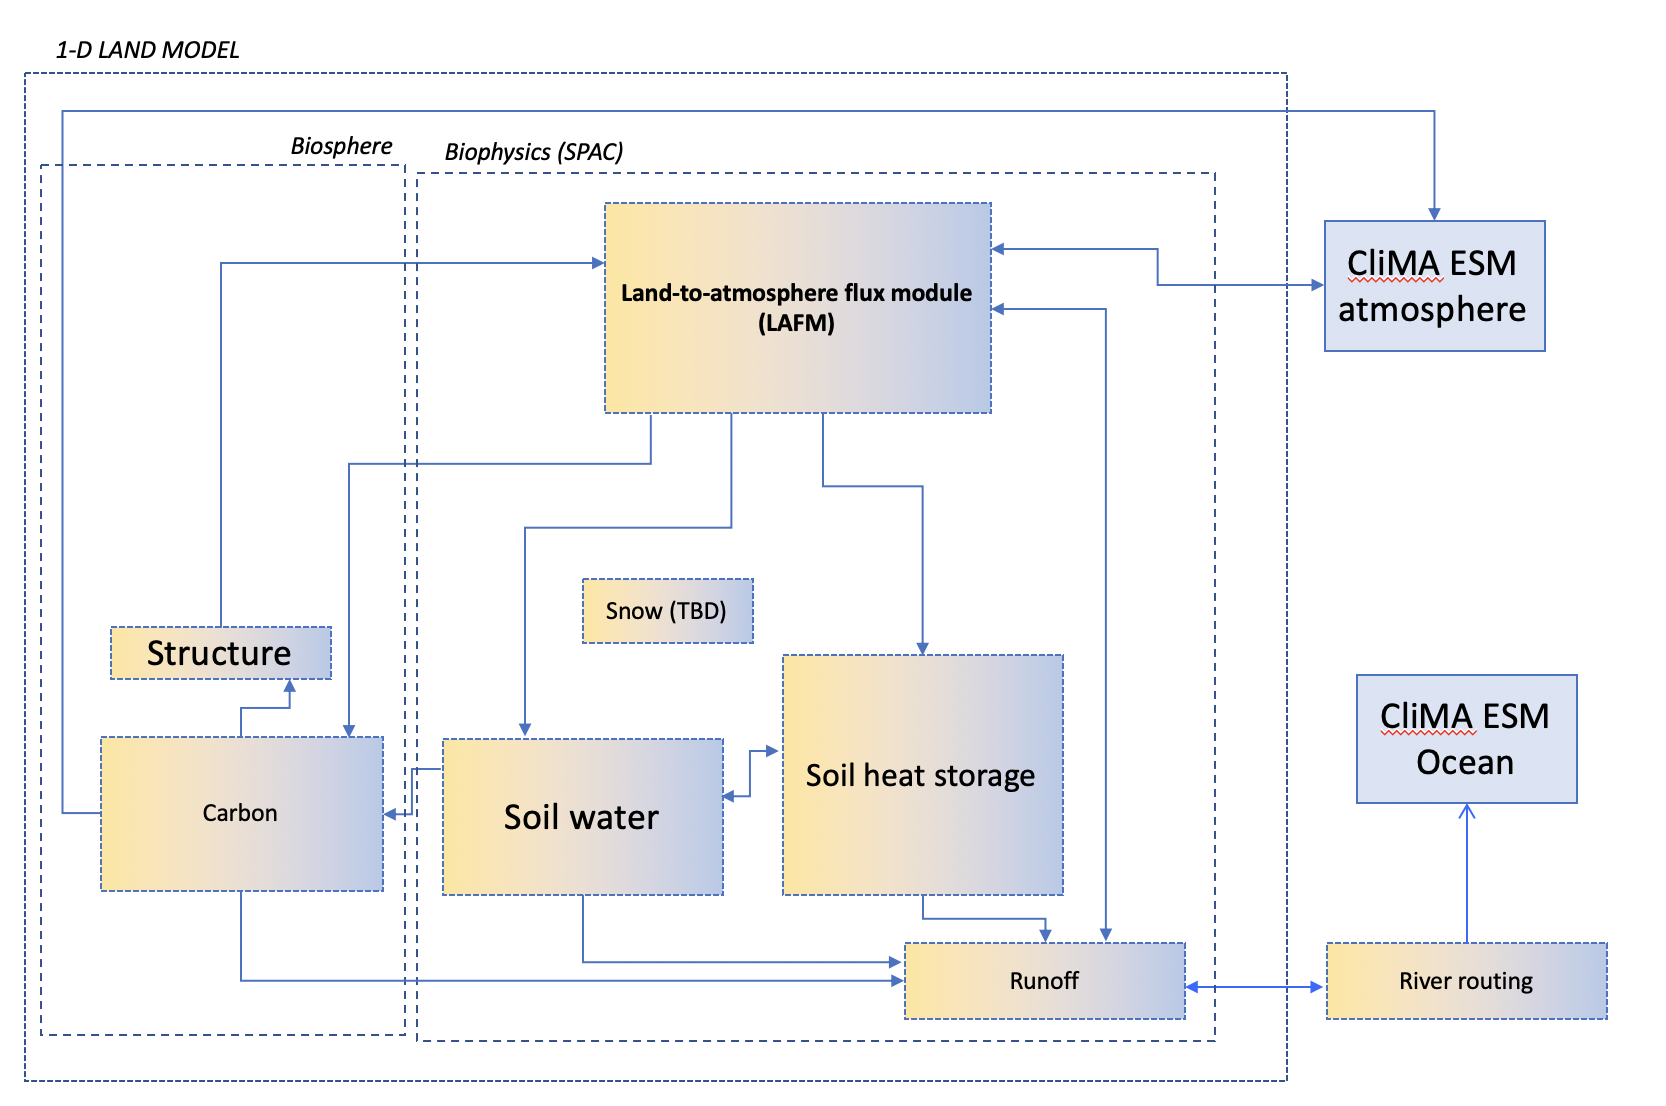
\includegraphics[width=\textwidth,height=\textheight,keepaspectratio]{CLIMA-land/LM_figures/JPLCLIMA_LM_DESIGN_20191115.png}
\caption{Schematic of land model modules and internal + external dependencies. [ALL: please comment + suggest improvements; Pierre's comment: SPAC should include all biophysics, re-name/re-arrange/simmplify boxes]}
\end{figure}
% Please add the following required packages to your document preamble:
% \usepackage{graphicx}
\begin{table}[]
\resizebox{\textwidth}{!}{%
\begin{tabular}{|l|l|l|l|}
\hline
Module [code]         & Input requirements [From]                                                                & Output requirements                                                       & Module requirements                      \\ \hline
Carbon [C]            & \begin{tabular}[c]{@{}l@{}}GPP [F], \\ Soil water profile [W], \\ Soil temperature profile [E]\end{tabular}                                                               & \begin{tabular}[c]{@{}l@{}}Carbon states\\ (Biomass, inc. foliar, roots, wood;\\ Dead organic C) \\ Carbon fluxes \\ (respiration, disturbance fluxes)\end{tabular} & \begin{tabular}[c]{@{}l@{}}The carbon module will calculate \\ internal land biosphere carbon transfers \\ (allocation, mortality, mineralization), \\ and gross land-atmosphere C fluxes \\ (respiration, fires)\end{tabular} \\ \hline

Structure [S]         & Biomass [C]                                                             & \begin{tabular}[c]{@{}l@{}}Biophysical states:\\ Canopy height, Chlorophyll, \\Root profile, LMA\end{tabular}                                                        &                                                                   \\ \hline
Soil water [H]        & \begin{tabular}[c]{@{}l@{}}Soil freeze/Thaw state [E] \\ Precipitation [A]\\ Evaporation [F], \\ Transpiration (vertically resolved), \\ root profile [S]\end{tabular} &
\begin{tabular}[c]{@{}l@{}}
Vertical soil water states\\Soil water fluxes\\Runoff\end{tabular}                                                                                                                  & \begin{tabular}[c]{@{}l@{}}Module will calculate vertical \\ water flow in soil Darcy’s law, \\ Richards equations, hydraulic \\redistribution,  runoff, etc.\end{tabular}                                                     \\ \hline
Soil heat storage [E] & Soil water [H], Precip. temp [A]


& 
\begin{tabular}[c]{@{}l@{}}
Vertical temperature profile\\
Runoff temperature       \end{tabular}                                               &                                                                                                \\ \hline
%%%%%%(SPAC-Flux)%%%%%
\begin{tabular}[c]{@{}l@{}}
Land-to-atmosphere\\ fluxes [F]  \\
(previously SPAC-Flux)

\end{tabular}

        & \begin{tabular}[c]{@{}l@{}}Atmospheric variables [A], \\ Biophysical states[S], \\ Soil water profile [H], \\ Soil energy profile [E],\end{tabular}                   & \begin{tabular}[c]{@{}l@{}}Land-surface Fluxes\\ GPP, evapotranspiration, H, $\lambda$E, L↑, S↑ \end{tabular}                                 & 

\begin{tabular}[c]{@{}l@{}} Canopy P interception\\ Radiative transfer in canopy     \end{tabular}                                                        \\ \hline

River routing [R]        & \begin{tabular}[c]{@{}l@{}} Soil runoff [H], \\ CliMA Ocean [O] \end{tabular}                             & \begin{tabular}[c]{@{}l@{}} River Discharge\end{tabular}                                             &                                     \\ \hline \hline \hline


CliMA Atmosphere [A]        & \begin{tabular}[c]{@{}l@{}}Land surface fluxes [F], \\ Land biosphere fluxes [C]\end{tabular}                             & \begin{tabular}[c]{@{}l@{}}Atmospheric variables [for land]\\ L↓, S↓, precip, temperature, humidity,\end{tabular}                                             &                                     \\ \hline

CliMA Ocean [O]        & \begin{tabular}[c]{@{}l@{}}River discharge [R] \end{tabular}                             & \begin{tabular}[c]{@{}l@{}} Ocean variables (for land) Sea Level\end{tabular}                                             &                                     \\ \hline

\end{tabular}%
}
\caption{\label{tab:LM-modules}Summary of module input, output & functional requirements. Comprehensive list of module inputs, outputs and equations are included in subsequent sections. [MISSING: snow module and associated dependencies. Ensure consistency with rest of CliMA framework]}
\end{table}


\section{Soil}

\subsection{Heat equation}
In the soil heat will be diffused following a 1D vertical heat diffusion:
\begin{equation}
     \frac{\partial (\rho_s c_s T_s) }{\partial t} = \frac{\partial }{\partial z}\lambda_s \frac{\partial T_s }{\partial z}
\end{equation}
where the density of the soil $\rho_{s}$ and the soil heat capacity $c_s$ make up the volumetric heat capacity (i.e. $C = \rho_s c_s$), $\lambda_{s}$ is the thermal conductivity of the soil. Both the thermal conductivity and the capacity of the soil are functions of the soil moisture content, $\theta$. Note that the diffusion coefficient, or $\alpha = \lambda_s/(\rho_s c_s)$, has much less moisture dependence because of a compensation of the dependence between $\lambda_s$ and $c_s$. 
For the conductivity we will first follow the CLM formulation: \\
The thermal and hydraulic properties of the soil are assumed to be weighted combinations of a mineral and organic layers of the soil (Lawrence and Slater 2008). The soil layer organic matter fraction $f_{om}$ is 
\begin{equation}
    f_{om} = \rho_{om}/\rho_{om,{\rm max}}
\end{equation}
The thermal conductivity is then $\lambda_s = K_e \lambda_{\rm sat} + (1-K_e) \lambda_{\rm dry}$, with $K_e$ is the Kersten number, a function of soil relative humidity $s=\theta/\theta_{\rm sat}$, with $\theta(x,y,z,t)$ the soil moisture content. Those functions are rather empirical. One example of which is $K_e = \exp \big( \gamma((1-s(\gamma-1.33))\big)$. For  the  deep  ground  layers  (typical  of  saturated  granitic  rock;  Clauser  and  Huenges,  1995) $\lambda_s =  \lambda_{\rm dry} = 3 \rm W  m^{-1}  K^{-1}$ as $K_e=0$.

The heat capacity of the soil is:
$c_s=\theta c_{\rm liq} + (1-\theta) c_{\rm dry}$, with $\theta$ the soil moisture content.[AAB + ML: this doesn't work in case of phase transition?]


The dry soil heat capacity is a weighted average of pure soil and organic matter heat capacity $c_{\rm dry} = (1-f_{om})c_{soil} + f_{om}c_{om}$ (Farouki, 1981).
$c_{soil} = {\rm \frac{2.128 (sand)+ 2.385 (clay)}{(sand) + (clay)}}$, with sand and clay the sand, clay percentage in the soil, respectively.
In the bedrock we take $c_{soil,bedrock} = 2 \cdot 10^6 {\rm J m^{-1} K^{-1}}$ as the heat capacity of the bedrock and $c_{s,om} = 2.5 ×10^6 {\rm J m^{-1} K^{-1}}$ the heat capacity of organic matter (Farouki, 1981).

\begin{table}[]
\resizebox{\textwidth}{!}{%
\begin{tabular}{lllll}
\hline
State Variables & Description   & Units     & Range & Example value \\ \hline
$T_s$       & Soil Temperature & K & 0 - $\infty$       & 286 K \\
$f_{om}$   & Organic Matter Fraction &   [\%]        &   0 - 100           &    3-6 \%       \\

\hline
Auxiliary State Variables & Description   & Units     & Range & Example value \\ \hline
$\partial T_s$ /  $\partial z$       & Soil Temperature Gradient & K/m & 0 - $\infty$       & 10 K/m \\
$K_e$  & Kersten Number &  [-] & 0 - 1  &   $\sim$0 for dry , $\sim$1 for wet soils      \\
$\gamma$ & [ ??? ] & [ ??? ] & [ ??? ]  &    [ ??? ]      \\

\hline
Constants (known) & Description   & Units     & Range & Example value \\ \hline
$\alpha_s$ =  $\lambda_s$ / $C_s$    & Thermal Diffusivity & m$^2$/s  & 0 - $\infty$       & 2e$^{-6}$ m$^2$/s \\
$\lambda_s$       & Soil Thermal Conductivity & W/(m K) & 0 - $\infty$       & 0.85 W/(m K) \\
$\lambda_{sat}$       & Saturated Thermal Conductivity & W/(m K) & 0 - $\infty$       & 0.35 W/(m K) \\
$\lambda_{dry}$       & Dry Thermal Conductivity & W/(m K) & 0 - $\infty$       & 1.5 W/(m K) \\

\hline
Constants (empirical) & Description   & Units     & Range & Example value \\ \hline
$\rho_s$       & Density of Soil & kg/m$^3$ & 0 - $\infty$       & 2.65 g/cm$^{3}$ or 2650 kg/m$^{3}$ \\
$c_s$       & Soil Heat Capacity & J/(kg K) & 0 - $\infty$       & 1000 J/(kg K) \\
$C_s$ =  $\rho_s$  $c_s$    & Volumetric Soil Heat Capacity & J/(m$^3$ K) & 0 - $\infty$       & 2e$^{9}$ J/(m$^3$ K) \\
$c_s,dry$       & Dry Soil Heat Capacity & J/(kg K) & 0 - $\infty$       & 800 J/(kg K) \\
$c_s,liq$       & Wet Soil Heat Capacity & J/(kg K) & 0 - $\infty$       & 1600 J/(kg K) \\
$c_s,bedrock$       & Heat Capacity at Bedrock Layer & J/(kg K) or J/(m K) & 0 - $\infty$       & 2e$^{6}$ J/(m K) [ ??? ] \\
$c_s,om$       & Heat Capacity of Organic Matter &  J/(kg K) or J/(m K) & 0 - $\infty$       & 2.5e$^{6}$ J/(m K) [ ??? ] \\
$\rho_{om}$ [ ??? ]  & Organic Matter Density & kg/m$^3$ & 0 - $\infty$       & 150 kg/m$^{3}$  \\
$\rho_{om,max}$ [ ??? ]  & Maximum Organic Matter Density &  kg/m$^3$ & 0 - $\infty$          &    2650 kg/m$^{3}$      \\

\hline
\end{tabular}%
}
\caption{List of heat eqs variables}
\end{table}

\begin{figure}[htb]
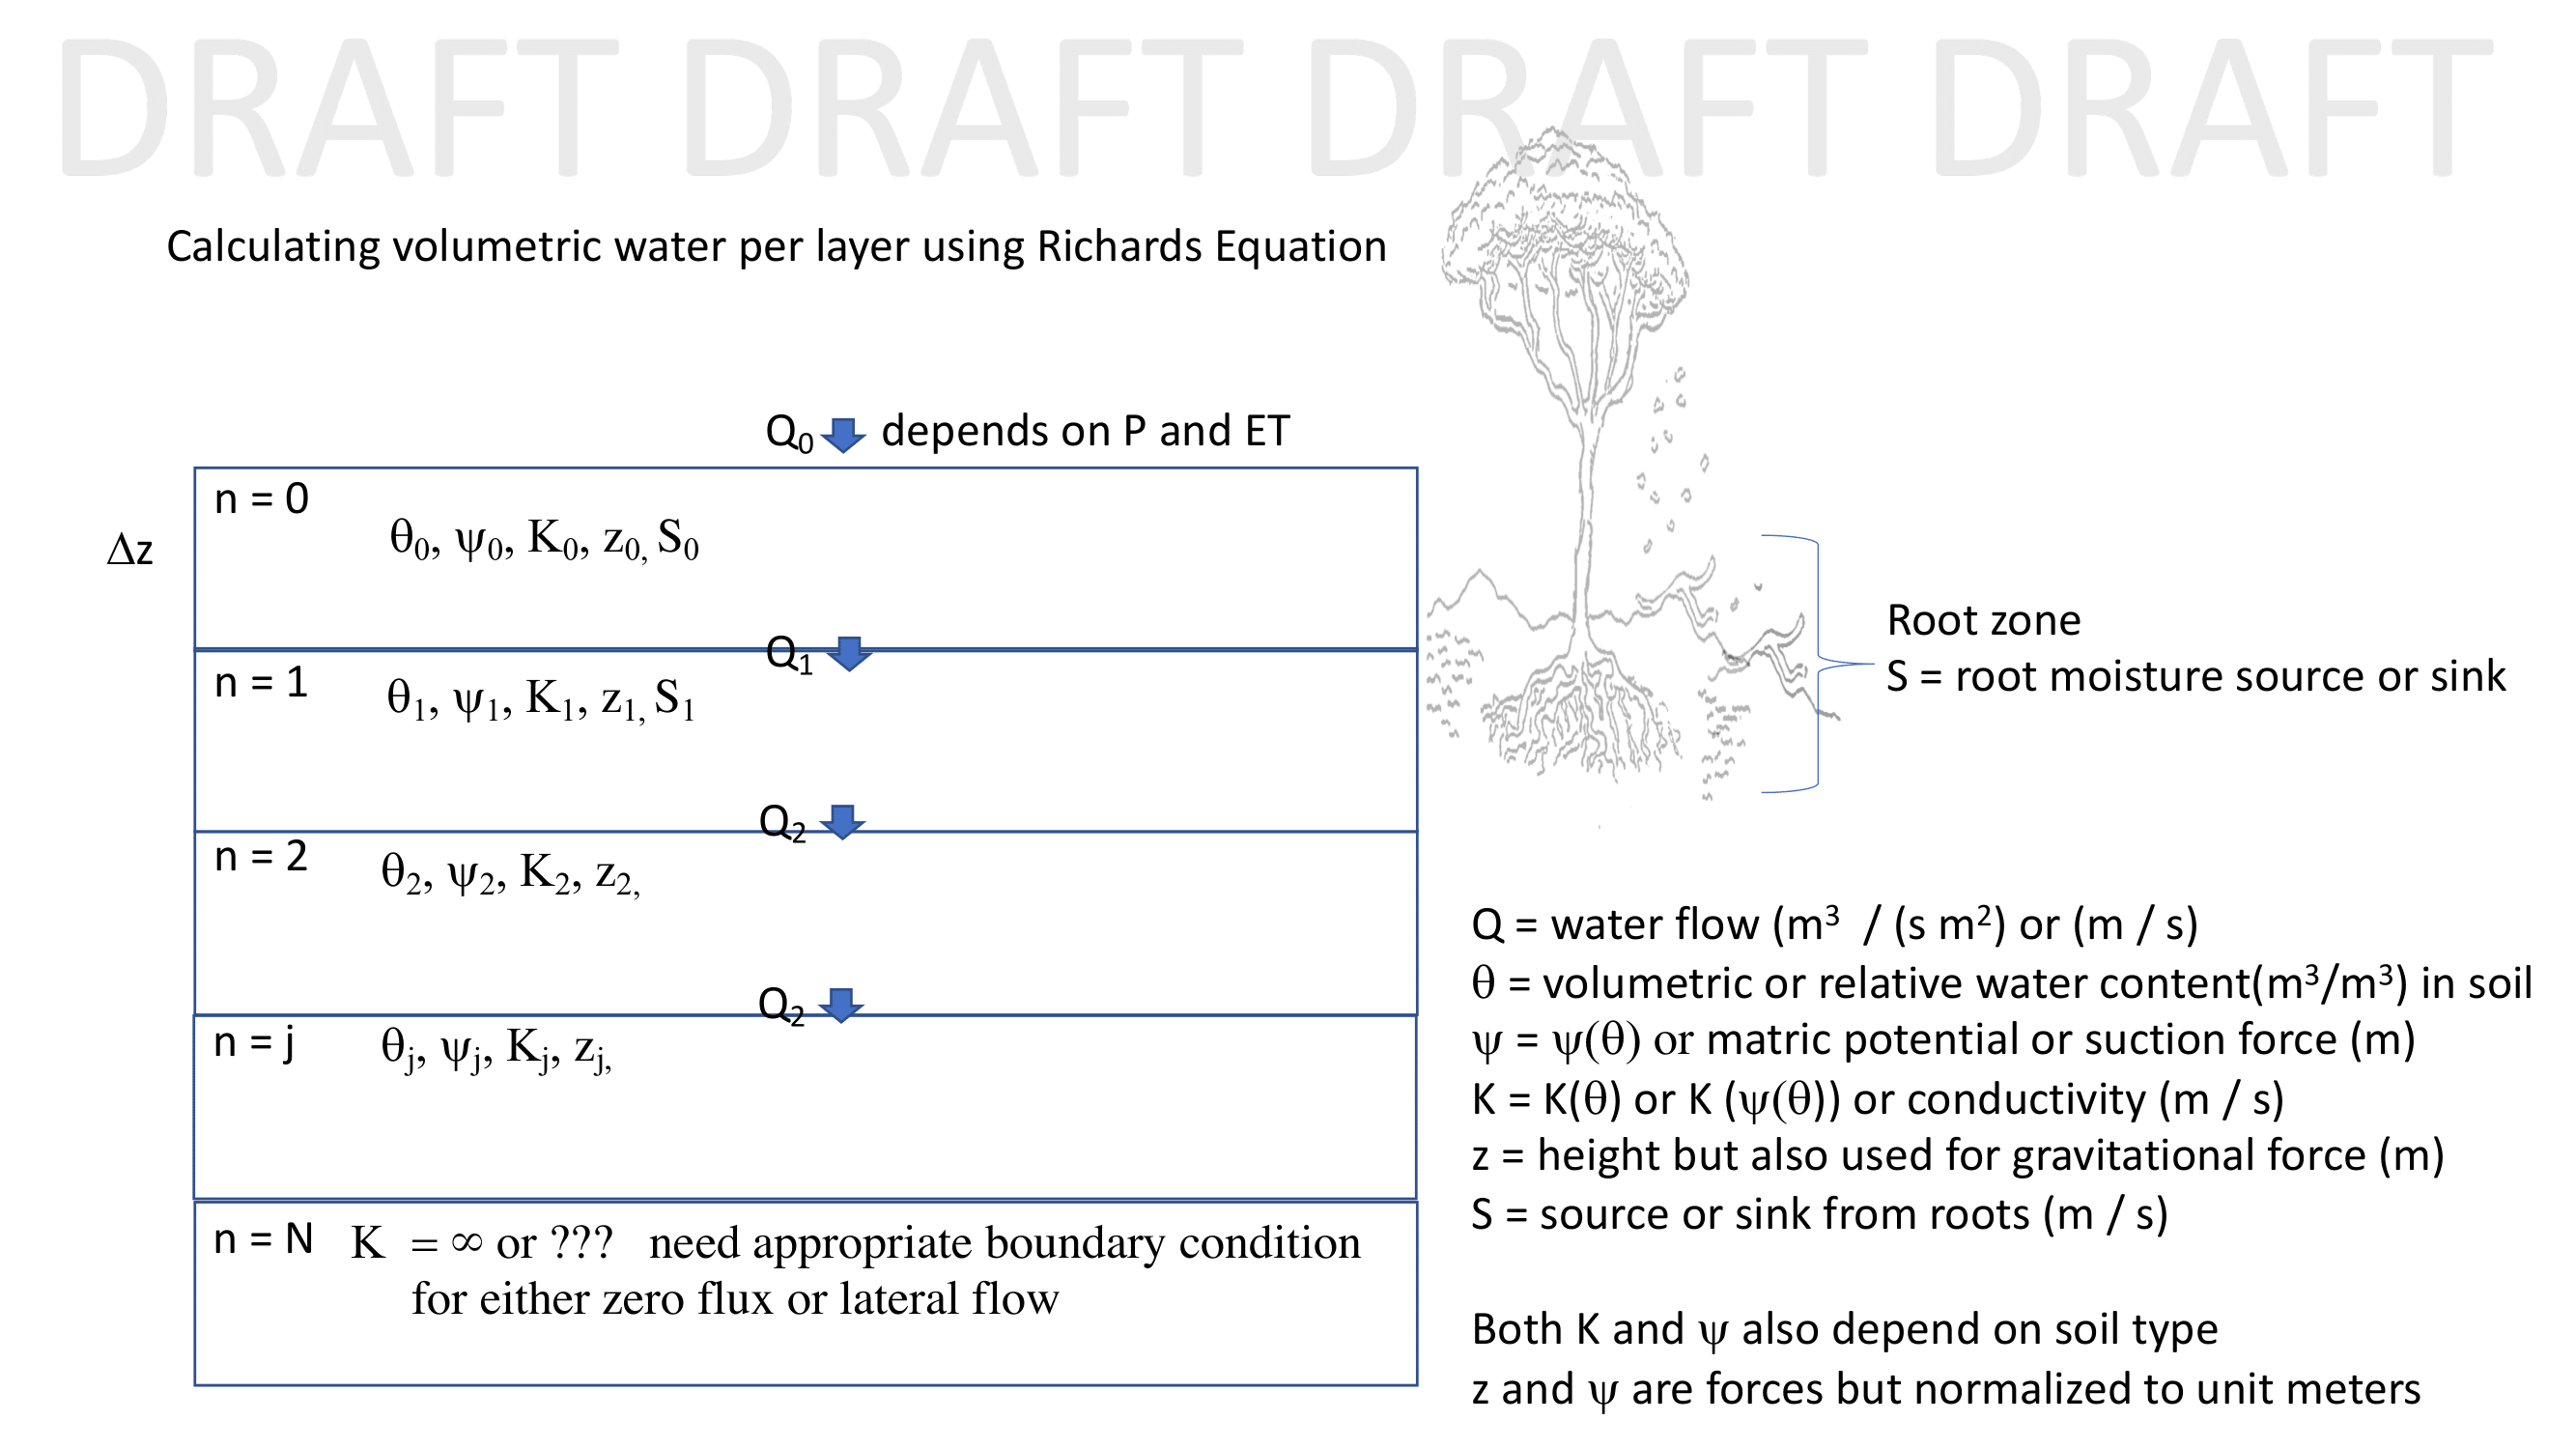
\includegraphics[scale=.15]{CLIMA-land/LM_figures/SoilSchematic-1.png}
\caption{Draft of soil schematic figure}
\end{figure}

\subsection{Moisture equation}
Moisture conservation is usually divided into two steps: 1) the unsaturated zone where total water storage is related to the relative water content $\theta$ and transport is typically assumed to be 1D in the vertical and 2) the saturated zone where water storage is related to changes in the water head through the storativity (porosity for an unconfined aquifer, and storativity for confined aquifer).
Let us start with the 3D Richards' equation so we do not lose generality (1D flow is just an approximation similar to shallow water equation). Water storage is written as $S$ (units of $m^3/m^3$). For instance in the unsaturated soil, the storage is related to the water content $S=\theta$. In an unconfined aquifer $dS=S_y dh$, with $S_y$ the unconfined aquifer specific yield, nearly equal to porosity $n$. Finally, in the confined aquifer $dS=S_s dh$, with $S_s$ the aquifer storativity. Note that the concept of aquifer storativity implicitly assumes a vertically-integrated Richards' equation over the thickness of the aquifer $b$. When resolving this vertically a choice might have to be made - TBD later.

Without loss of generality we can therefore write the storage as a (nonlinear) function of the head 
\begin{equation}
     h=z+\psi
\label{head}
\end{equation}

, with $\psi$ the matric potential so that $dS = C(\psi)d\psi$. In the unsaturated case C($\psi$)=$\partial \theta /\partial h$ \\ and in the saturated (unconfined aquifer) case it is the specific yield $C(\psi)=S_y$.
We therefore write the conservation of mass including sinks/sources (such as due to roots but also for instance non-local transport due to preferential flow). 
So the generic 3D Richards' equation using chain's rule:
\begin{equation}
     \frac{\partial S}{\partial t} = C(\psi)\frac{\partial \psi}{\partial t} = -\nabla \cdot {\bf{q}} + {\rm Source}
\label{Richards}
\end{equation}
with $\bf{q}$ Darcy's flow, with 
\begin{equation}
     \bf{q} = - \mathbf{K}(\psi) \otimes \nabla h
\end{equation} with $ \mathbf{K}$ the hydraulic conductivity tensor, and $\otimes$ the tensor product.
For simplicity we will assume that the flow is isotropic and therefore along the head gradient (this might not be true because of the strong horizontal layering of the soil creating important anisotropy; this could be relaxed later):
\begin{equation}
     {\bf{q}} = - K \ \nabla h
\end{equation}
So we are left with our simplified Richards' 3D equation:
\begin{equation}
     C(\psi)\frac{\partial \psi}{\partial t}  = \nabla \cdot \left( {K(\psi) \nabla h} \right) + {\rm Source}
\label{Richards_simple}
\end{equation}
Equation (\ref{Richards_simple}) written in head term is continuous across saturation interfaces.
We finally write this in terms of $\psi$ only
\begin{equation}
     C(\psi)\frac{\partial \psi}{\partial t}  = \nabla \cdot \left( {K \nabla \psi} + K \right) + {\rm Source}
\label{Richards_simple}
\end{equation}


In the unsaturated zone, the storage is simply $S=\theta$, yet we will keep a head-based approach for continuity. $\theta$ is related to $h$ though the so-called retention curves (assuming negligible hysteresis). The potential options for the retention curves are discussed in section \ref{SoilMoisture:Retention_Curves}

Therefore in the unconfined aquifer we will have 
\begin{equation}
     \frac{\partial \theta}{\partial \psi}\frac{\partial h}{\partial t} = \nabla \cdot \left( {K(\psi) \nabla \psi} + K(\psi) \right) + {\rm Source}
\label{Richards_simple_uns}
\end{equation}
This is then solved typically in the vertical and simplifies to:
\begin{equation}
     \frac{\partial \theta}{\partial \psi}\frac{\partial \psi}{\partial t} = \frac{\partial}{\partial z}  \left( {K \frac{\partial \psi}{\partial z} + K(\psi)} \right) + {\rm Source}
\label{Richards_simple_uns_1D}
\end{equation}
with $K(\psi)$, an exponential function of $\psi$.
We note however that as the horizontal resolution becomes finer and in the presence of rain this assumption is not tenable anymore.

ADD A NOTE - COULD IT BE BETTER TO SOLVE BY DIRECTLY DIVIDING BY dTHETA/DPSI so THAT WE HAVE A DICUSSIION WHICH IS VERY SMOOTH

In an unconfined aquifer, then we will simply replace the storage change by a specific yield $S_y$ (normalized by the aquifer depth):
\begin{equation}
     \frac{\partial S}{\partial t} = S_y \frac{\partial h}{\partial t}  
\end{equation}
this will lead to the following equation:
\begin{equation}
     \frac{\partial S}{\partial t} = S_y \frac{\partial h}{\partial t} = \nabla \cdot \left( {K_{\rm sat} \nabla h} \right) + {\rm Source}
\label{Richards_simple}
\end{equation}
with $K_{\rm sat}$ the saturated hydraulic conductivity. 


\begin{table}[]
\resizebox{\textwidth}{!}{%
\begin{tabular}{lllll}
\hline
State Variables & Description   & Units     & Range & Example value \\ \hline
$S$       & Water Storage                    & m$^3$/m$^3$ & 0 - 1 & 0.43 m$^3$/m$^3$       \\
$b$       & Aquifer Thickness  & m &  0 - $\infty$  & 10 m        \\


\hline
Auxiliary State Variables & Description   & Units     & Range & Example value \\ \hline
$\theta$       & Relative Water Content                    & m$^3$/m$^3$ & 0 - 1       & 0.2 m$^3$/m$^3$ \\
$\psi$       & Matric Potential  & m or kPa &  $-\infty$ - $\infty$  & 10 m or 100 kPa       \\
$h$       & Hydraulic Head  & m or kPa &  $-\infty$ - $\infty$    & 10 m or 100 kPa     \\
$z$       & Height or Depth & m  &  0 - $\infty$    & 10 m     \\
$\bold{q}$       & Darcy's Flow  & m$^3$/s &  0 - $\infty$   & 1e$^{-6}$ m$^3$/s     \\


\hline
Constants (known) & Description   & Units     & Range & Example value \\ \hline
$S_{y}$       & Unconfined Aquifer Specific Yield   & m$^3$/m$^3$ &  0 - 1   & 0.2 m$^3$/m$^3$     \\
$S_{s}$       & Aquifer Storativity   & m$^3$/m$^3$ &  0 - 1 & 0.25 m$^3$/m$^3$       \\
$K$   & Hydraulic Conductivity &   m/s or cm/day       &    0 - $\infty$ & 0.1 cm/day    \\
$K_{sat}$   & Saturated Hydraulic Conductivity &   m/s or cm/day       &    0 - $\infty$ & 10 cm/day                    \\
$n$       & Porosity   & m$^3$/m$^3$  &   0 - 1  & 0.45 m$^3$/m$^3$     \\


\hline
Constants (empirical) & Description   & Units     & Range & Example value \\ \hline
$\theta_{r}$       & Residual Water Content   & m$^3$/m$^3$ & 0 - 1       & 0.05 m$^3$/m$^3$ \\
$\theta_{s}$       & Saturated Water Content   & m$^3$/m$^3$ & 0 - 1       & 0.45 m$^3$/m$^3$ \\
$\alpha$   & VG Scale Parameter for Retention Function & cm$^{-1}$ & 1e$^{-6}$ - 1e$^{-4}$  & 1e$^{-5}$ cm$^{-1}$ \\
$n$   & VG Shape Parameter for Retention Function & (-) & 4.0 - 8.0  & 7.1 \\
$L$   & VG Empirical Parameter for Retention Function & (-) & 0 - 1  & 0.5 \\
$S_{e}$   & Relative Degree of Saturation of the Soil & (-) & 0 - 1  & 0.25 \\



\hline
\end{tabular}%
}
\caption{List of moisture eqs variables [eventually maybe split into "states" and "parameters" tables]}
\end{table}

\subsection{Retention curves $\theta=f(\psi)$ and $K(\psi)$ in the unsaturated zone}
\label{SoilMoisture:Retention_Curves}
\subsubsection{Van Genuchten}
We will use the van Genuchten's formulation which is better behaved in saturated conditions than the Brooks and Corey relationship 
\begin{equation}
     \theta(\psi) = \theta_r + \frac{\theta_s - \theta_r}{\left[ 1+(\alpha |\psi|)^n \right]^{m}}
\end{equation}
with $m=1-1/n$.
For hydraulic conductivity, we have
\begin{equation}
     K(\psi) = K_{s} S_e^L \left (1 -  (1-S_e^{1/m})^m  \right)^2
\end{equation}
with $L$ an empirical parameter assumed to be $L=0.5$. $S_e$ is the relative degree of saturation of the soil and $K_{s}$ the hydraulic conductivity at saturation. 
\begin{equation}
     S_e = \frac{\theta(\psi) - \theta_r}{\theta_s - \theta_r}
\end{equation}
The derivative of $\theta$ with respect to $\psi$, $C(\psi)$ is:
\begin{equation}
     \frac{\partial \theta}{\partial \psi} =   \frac{m n\alpha^n |\psi|^{n-1}}{\left[ 1+(\alpha |\psi|)^n \right]^{m+1}} \left( \theta_s - \theta_r \right) 
\end{equation}



\subsubsection{Brooks and Corey}
\begin{equation}
     S_e = \frac{\theta(\psi) - \theta_r}{\theta_s - \theta_r} = \left( \frac{\psi}{\psi_{ae}}\right)^{-\lambda}
\end{equation}
with $\psi_{ae}$ the air entry point.
\begin{equation}
     K_s = \left( \frac{\psi}{\psi_{ae}}\right)^{-2-3\lambda}
\end{equation}





\subsection{Technical note: continuity of Richards' equation at the unsaturated-saturated interface}
We note that there is a fundamental issue in the continuity of the Richards' equation at the water table interface. Indeed, $C(\psi)$ goes to zero at the bottom of the unsaturated zone but is a fixed value in the saturated zone (the specific yield), leading to sharp derivative discontinuity. We note that the specific yield is empirical, mainly based on measurements and is close to the soil moisture content at saturation $\theta_s$. We will return to this.

We write the porous medium temporal mass $M$ balance per unit volume as a departure from the hydrostatic pressure, equivalent to $\partial h/\partial z=0$, with $h=z+\psi$. The temporal departure from hydrostatic balance is written as $\psi'$ with corresponding changes in density $\rho'=\rho-\overline\rho$. The water porous medium density conservation reads:
\begin{equation}
\frac{\partial \rho \theta}{\partial t} = {\overline{\rho}} \nabla \cdot \left( K(\psi) \left( \nabla \psi + {\mathbf e_z} \right) \right)
\end{equation}
In which we have neglected the mass of water vapor.
We expand this into:
\begin{equation}
{\overline \rho} \frac{\partial \theta}{\partial t} + \theta \frac{\partial \rho}{\partial t} = {\overline \rho} \nabla \cdot \left( K(\psi) \left( \nabla \psi + {\mathbf e_z} \right) \right)
\end{equation}
Dividing by $\overline \rho$ gives:
\begin{equation}
\frac{\partial \theta}{\partial t} + \frac{\theta}{\overline \rho} \frac{\partial \rho}{\partial t} = \nabla \cdot \left( K(\psi) \left( \nabla \psi + {\mathbf e_z} \right) \right)
\end{equation}
This equation looks like the unsaturated Richards’ equation beside the presence of the second term on the left hand side, related to the compressibility of liquid water: $ \frac{\theta}{\overline \rho} \frac{\partial \rho}{\partial t}$.

We now use chain’s rule with respect to variations in internal pressure $\psi$ but do not assume that liquid water is incompressible, to write the mass change:
\begin{equation}
{\overline \rho} \frac{\partial \theta}{\partial t} + \theta \frac{\partial \rho}{\partial t} 
\end{equation}

In the unsaturated zone the second term on the lhs is negligible. In the saturated zone, the converse is true and the density term becomes important. At the water table interface, the $\theta=\theta_s=n$, the porosity assumed to be the same as the saturation water content $\theta_{s}$. We therefore further write $\theta$ in terms of the relative saturation content $s=\theta/\theta_s$.
The liquid water mass balance can be written
\begin{equation}
\underbrace{{\overline \rho} n \frac{\partial s}{\partial t} }_\text{\rm unsaturated mass change} + \underbrace{{\overline \rho} s \frac{\partial n}{\partial t}  }_\text{\rm change in porous medium porosity}  
+ 
\underbrace{\theta \frac{\partial \rho}{\partial t}   }_\text{\rm change in liquid water density}  
\label{mass_balance:split}
\end{equation}
The change in density (assuming negligible temperature and solute impact) can be written:
\begin{equation}
\frac{\partial \rho}{\partial t} = \rho \beta \frac{\partial \psi}{\partial t}
\end{equation}
with $\psi$ the pressure.
Assumed an elastic material (and neglecting the change in density of the material) (Bear 2018) and introducing the coefficient of porous medium compressibility $\alpha_{pm}$, with assumed veritcal stress:
\begin{equation}
\alpha_{pm}=\frac{1}{V_{pm}} \frac{\partial V_{pm}}{\partial \sigma_z} = \frac{1}{1-n} \frac{\partial n}{\partial \psi}
\end{equation}
with $\sigma_z$ the stress tensor in the vertical direction.
This then lead to the change in porosity due to the porous medium compaction:
\begin{equation}
\frac{\partial n}{\partial t} = (1-n)\alpha_{pm}\frac{\partial \psi}{ \partial \psi}
\end{equation}
The combined change in mass of the porous medium water can be finally written using equation (\ref{mass_balance:split}) 
\begin{equation}
\frac{\partial \theta \rho}{\partial t} = 
\underbrace{n \rho \frac{\partial s}{ \partial t} }_\text{\rm unsaturated mass change} + \underbrace{s \rho \left[  (1-n)\alpha_{pm} + n\beta \right] \frac{\partial \psi}{\partial t} }_\text{\rm saturated mass change}
\end{equation}
We note here that we made a convenient approximation: we used the matric potential $\psi$, instead of the pressure $p$. The rational for that is that far away from the water table the unsaturated term the left hand side domaintes. Within the saturated zone, far from the water table, the lhs vanishes. Yet an advantage is that the equation bcomes continuous at the interface, with continuous and non-vanishing temporal derivatives. Another way to think about this is that the fluid is composed of a mixture of saturated and saturated water at the interface - i.e the interface is not abrupt. 
Our master equation for the porous medium water conservation then becomes:
\begin{equation}
 \left( n \rho \frac{\partial s}{\partial \psi} + s \rho   (1-n)\alpha_{pm} + s n\beta \right) \frac{\partial \psi}{\partial t} = \rho \nabla \cdot \left( K(\psi) \left( \nabla \psi + {\mathbf e_z} \right) \right)
\label{master_equation_porous_medium}
\end{equation}
or dividing by $\rho$
\begin{equation}
\red{ n \left(  \frac{\partial s}{\partial \psi} + s \frac{1-n}{n}\alpha_{pm} + s \beta \right) \frac{\partial \psi}{\partial t} = \nabla \cdot \left( K(\psi) \left( \nabla \psi + {\mathbf e_z} \right) \right)}
\label{master_equation_porous_medium}
\end{equation}







We now integrate the mass balance equation over the depth of the unconfined aquifer i.e. from $z=z_0$ to $z=h+\epsilon$ (with $z=z_0$ the bedrock elevation – not necessarily 0):
\begin{equation}
\int_{z_0}^{h+\epsilon} { n \left(  \frac{\partial s}{\partial \psi} + s \frac{1-n}{n}\alpha_{pm} + s \beta \right) \frac{\partial \psi}{\partial t}  dz = \int_{z_0}^{h+\epsilon} \nabla \cdot \left( K(\psi) \left( \nabla \psi + {\mathbf e_z} \right) \right)} dz
\end{equation}
\begin{equation}
\int_{z_0}^{h+\epsilon} { n \left(  \frac{\partial s}{\partial \psi} + s \frac{1-n}{n}\alpha_{pm} + s \beta \right) \frac{\partial \psi}{\partial t}  dz =
K(\psi) \left( \frac{\partial \psi}{\partial z} + 1 \right)_{|z=h+\epsilon} + \nabla_H \cdot \int_{z_0}^{h+\epsilon}  K(\psi) \nabla_H \psi dz
\end{equation}
Using Leibniz rule, the lhs can be written as 
\begin{equation}
\frac{\partial \int_{z_0}^h \rho \theta_s dz }{\partial t} - \rho \theta_s \frac{\partial h}{\partial t}=
K(\psi) \left( \frac{\partial \psi}{\partial z} + 1 \right)_{|z=h+\epsilon} \\
+ \nabla_H \cdot \int_{z_0}^{h+\epsilon}  K(\psi) \nabla_H \psi dz
\end{equation}
The rhs can be rewritten as:
\begin{equation}
\int_{z_0}^h  \nabla \cdot \left( {\overline \rho} K(\psi) \left(\nabla \psi + {\mathbf e_z} \right) \right) dz = {\overline \rho} K(\psi) \left(\nabla \psi + {\mathbf e_z} \right)_{|h}  + \int_{z_0}^h  \nabla_H \left( {\overline \rho} K(\psi) \left(\nabla_H \psi \right) \right) dz
\end{equation}

Because the rate of change of the water table is much larger than the changes in density, we have: 
\begin{equation}
-	\theta_s \frac{\partial h}{\partial t} = 
 K(\psi) \left(\nabla \psi + {\mathbf e_z} \right)_{|h}  + \int_{z_0}^h  \nabla_H \left( {\overline \rho} K(\psi) \left(\nabla_H \psi \right) \right) dz
\end{equation}

Using the total derivative of $\theta$, we can write:


Dupuit–Forchheimer assumptions: flow is nearly 2D below the water table (similar to shallow water approximation) and hydrostatic i.e. $\partial h/\partial z=0$.

\subsection{Summary of soil heat and moisture equations for CliMA implementation}

This section contains a summary of all equations needed for implementation of the soil heat and moisture equations into CliMA. All variables are defined 

[OPTION: list equations in table for succinct description and avoid extra equation numbers in document] \\

\textbf{Soil Heat Equations} \\


\begin{equation}
     \frac{\partial (\rho_s c_s T_s) }{\partial t} = \frac{\partial }{\partial z}\lambda_s \frac{\partial T_s }{\partial z}
\end{equation}

\begin{equation}
    f_{om} = \rho_{om}/\rho_{om,{\rm max}}
\end{equation}


\begin{equation}
\lambda_s = K_e \lambda_{\rm sat} + (1-K_e) \lambda_{\rm dry}
\end{equation}

\begin{equation}
K_e = \exp \big( \gamma((1-s(\gamma-1.33))\big)
\end{equation}

\begin{equation}
s=\theta/\theta_{\rm sat}
\end{equation}

\begin{equation}
c_s=\theta c_{\rm liq} + (1-\theta) c_{\rm dry}
\end{equation}

\begin{equation}
c_{\rm dry} = (1-f_{om})c_{soil} + f_{om}c_{om}
\end{equation}

\begin{equation}
c_{soil} = {\rm \frac{2.128 (sand)+ 2.385 (clay)}{(sand) + (clay)}}
\end{equation}  \\



\textbf{Soil Moisture Equations} \\

(Unsaturated soil)
\begin{equation}
 dS=\theta 
\end{equation}

(Saturated - Unconfined Aquifer)
\begin{equation}
 dS=S_y dh ; S_y = n
\end{equation}

(Saturated - Confined Aquifer)
\begin{equation}
 dS=S_s dh
\end{equation}

\begin{equation}
 h=z+\psi
\end{equation}

\begin{equation}
dS = C(\psi)d\psi
\end{equation}

(Unsaturated soil)
\begin{equation}
C(\psi)=\partial \theta /\partial h 
\end{equation}

(Saturated  - Unconfined Aquifer)
\begin{equation}
C(\psi)=S_y 
\end{equation}

\begin{equation}
     \frac{\partial S}{\partial t} = C(\psi)\frac{\partial \psi}{\partial t} = -\nabla \cdot {\bf{q}} + {\rm Source}
\label{Richards}
\end{equation}

\begin{equation}
     \bf{q} = - \mathbf{K}(\psi) \otimes \nabla h
\end{equation}

\begin{equation}
     {\bf{q}} = - K \ \nabla h
\end{equation}

\begin{equation}
     C(\psi)\frac{\partial \psi}{\partial t}  = \nabla \cdot \left( {K(\psi) \nabla h} \right) + {\rm Source}
\label{Richards_simple}
\end{equation}

\begin{equation}
     C(\psi)\frac{\partial \psi}{\partial t}  = \nabla \cdot \left( {K \nabla \psi} + K \right) + {\rm Source}
\label{Richards_simple}
\end{equation}

\begin{equation}
     \frac{\partial \theta}{\partial \psi}\frac{\partial h}{\partial t} = \nabla \cdot \left( {K(\psi) \nabla \psi} + K(\psi) \right) + {\rm Source}
\label{Richards_simple_uns}
\end{equation}

\begin{equation}
     \frac{\partial \theta}{\partial \psi}\frac{\partial \psi}{\partial t} = \frac{\partial}{\partial z}  \left( {K \frac{\partial \psi}{\partial z} + K(\psi)} \right) + {\rm Source}
\label{Richards_simple_uns_1D}
\end{equation}

(Saturated - Unconfined Aquifer)
\begin{equation}
     \frac{\partial S}{\partial t} = S_y \frac{\partial h}{\partial t}  
\end{equation}

\begin{equation}
     \frac{\partial S}{\partial t} = S_y \frac{\partial h}{\partial t} = \nabla \cdot \left( {K_{\rm sat} \nabla h} \right) + {\rm Source}
\label{Richards_simple}
\end{equation} \\


\textbf{Retention functions for unsaturated soils - van Genuchten} \\


\begin{equation}
     \theta(\psi) = \theta_r + \frac{\theta_s - \theta_r}{\left[ 1+(\alpha |\psi|)^n \right]^{m}}
\end{equation}

\begin{equation}
m=1-1/n
\end{equation}

\begin{equation}
     K(\psi) = K_{s} S_e^L \left (1 -  (1-S_e^{1/m})^m  \right)^2
\end{equation}

\begin{equation}
L = 0.5
\end{equation}

\begin{equation}
     S_e = \frac{\theta(\psi) - \theta_r}{\theta_s - \theta_r}
\end{equation}

\begin{equation}
     \frac{\partial \theta}{\partial \psi} =   \frac{m n\alpha^n |\psi|^{n-1}}{\left[ 1+(\alpha |\psi|)^n \right]^{m+1}} \left( \theta_s - \theta_r \right) 
\end{equation}






\section{Land Boundary conditions}
We first discuss the heat boundary conditions for the soil medium.
\subsection{Ground heat flux at depth}
The bottom boundary condition for the soil will be assumed to be a vanishing ground heat flux $G=0$ at the bottom of the deepest soil layer. This will avoid specifying a constant temperature which would generate an artificial ground heat flux. Initialization will be based on preindustrial annual mean temperature for the soil profile to avoid too long spin up times.

\subsection{Surface energy budget}
The surface heat condition is a mixed boundary condition as it involves resolving the surface energy budget (SEB). The SEB including the canopy air heat capacity can write:
\begin{equation}
    \int_0^h{C_{air}dz \frac{\partial T_{air}(z)}{\partial t}} = R_n - G_0 - H - L_vE - GPP 
\end{equation}
with $C_{air}$ the specific heat of the air, $h$ the vegetation height, $R_n$ the net radiation at the top of the canopy, $G_0$ the ground heat flux at $z$=0, $H$ the sensible heat flux at the top of the canopy, $L_vE$ the latent heat flux at the top of the canopy and $GPP$ gross primary productivity within the canopy (a small but non-negligible term). Note that this neglect heat flux on stems (can be as large as ground heat flux but still need to be explored more carefully).

 The SEB will be solved for the skin temperature at the leaf/soil interface. To do so we will use a multi-layer canopy and a soil layer.
 The total SEB is then split into two components: the soil and canopy ones, allowing the resolution of the vegetation and soil temperatures.
 
\subsubsection{Soil surface energy budget}
The soil SEB is simply:
\begin{equation}
     R_{n,s} - G_0 - H_s - L_vE_s = 0  
     \label{SEB:soil}
\end{equation}
with $R_{n,s}$ the surface soil net radiation, $H_s$ the soil sensible heat flux, and $L_vE_s$ the soil latent heat flux.

\subsubsection{Vegetation surface energy budget}
The vegetation budget in turn is:
\begin{equation}
     R_{n,v} - G_v - H_v - L_vE_v - GPP = 0  
     \label{SEB:veg}
\end{equation}
with $R_{n,s}$ the vegetation net radiation, $H_s$ the vegetation sensible heat flux, $L_vE_s$ the vegetation latent heat flux, and $G_v$ the trunk heat flux, assumed to be negligible. 

At the leaf surface in the canopy, we will use a multi-layer canopy budget
\begin{equation}
    \int_z^{z+\delta z}{C_v (LM_d+S_d) dz\frac{\partial T_v}{\partial t}} = R_{n,v}(z) -H_v(z)-L_vE(z)-GPP(z)
\end{equation}
with $LM_d$ the mass vertical density of leaves, related to the leaf mass area and therfore to the lead area index density $LAId$, and leaf specific mass $LM$. $S_d$ is the stem mass vertical density.
(Note that the atmosphere will have to see the sensible and latent heat fluxes but we leave the atmosphere component as part of the atmospheric module). Note importantly that the canopy is considered as a dense canopy, i.e. like a porous medium so not all space can be filled up with air because of the stems and canopy volume. This will require some correction factor in the mass and energy conservation in the atmosphere at the top of the canopy for continuity (Schmid et al., 2019).

\subsection{Surface evapotranspiration}
Surface evapotranspiration is composed of four terms: 1. open-water body evaporation (e.g. lakes), 2. soil evaporation, 3. Plant canopy transpiration and 4. Canopy interception
\subsubsection{Open-water evaporation}
The open water body evaporation will simply use the same formulation as the ocean model (including waves).
\subsubsection{Soil evaporation}
Soil evaporation modeling has typically been relatively empirical leading to systematic issues with soils either drying much too fast or too slowly. We here use a recent formulation (Lehmann et al., 2019) informed by observations from either laboratory or in situ flux observations (Merlin et al. 2018). This formulation is aimed at modeling the evaporative front and its impact on soil evaporation. 
Soil evaporation then is 
\begin{equation}
    E_s = \rho \frac{e_s(T_s)-e_{a,s}}{r_{a,s}+r_{\rm shell}+r_{\rm soil}}
\end{equation}
with $e_{a,s}$ the near surface air vapor pressure, $r_{a,s}$ the surface aerodynamic resistance between the surface and near surface level, composed of a viscous boundary layer resistance $\delta /D_{air}$, with $\delta$ the depth of the viscous boundary layer (note that reality is trickier with a buffer regime - matching the viscous and turbulent layers). It should not be a major issue as this resistance will typically not be the primary limitation. The vapor shell resistance $r_{\rm shell}$ is due to the configurational resistance to diffusion through vapor shells forming around evaporating pores i.e. diffusion in 3-D from the evaporating pores across a hemisphere (Bange, 1953; Schlünder, 1988).
\begin{equation}
    r_{\rm shell} = \frac{1}{D_{\rm air}}\frac{\overline{r_{\rm pore}}(\pi-2\sqrt{\theta(z=0)})}{4\theta(z=0)}
\end{equation}
with mean pore size $\overline{r_{\rm pore}}$.
The soil resistance is related to the evaporative font and Darcy's law of capillarity effects.
\begin{equation}
    r_{\rm soil} = \frac{1}{4 K_s(\theta(z=0))\frac{\Delta H}{\Delta Z}}\frac{e_s(T_s)-e_{a,s}}{\rho}
\end{equation}
with $\frac{\Delta H}{\Delta Z}$ the head across a layer $\Delta Z$ (surface acppilarity effects between the wet subsurface and dry surface). It can be shown that (Lehmann et al., 2008; 2019) that 
\begin{equation}
   \frac{\Delta H}{\Delta Z} = \frac{L_{\rm gravity}}{L_{\rm capillarity}} = 1+E_0/(4K_s(h_c))
\end{equation}
with $E_0$ thes surface potential evaporation (i.e. in the absence of shell and soil resistances) “gravity length” $L_{\rm gravity}$ (difference between air entry value $h_b$ and critical capillary pressure head $h_c$ at which hydraulic flow paths become disconnected) with $h_c$ obtained from van Genuchten as:
\begin{equation}
   h_c = \frac{1}{\alpha}\left( \frac{n-1}{n} \right)^{\left( \frac{1-2n}{n} \right)}
\end{equation}

\subsubsection{Canopy reevaporation}
Interception of rainwater by the canopy remains highly empirical and few parameterizations exist. Those parameterization are not physically based and were tested at only very few sites. We are currently developing a method that should be able to give much better estimates of rainfall interception using hybrid machine leaning approaches, showing a clear dependence on rainfall maximum and Leaf Area Index. FOR LATER

\subsubsection{Transpiration}
Transpiration will follow an approach based on optimal stomatal behavior, which assumes that stomata are maximizing carbon uptake while minimizing water losses through transpiration (see photosynthesis section). 
Since we will use a multi-layer canopy we will always consider as the air reference value, the air in the vicinity of the leaves and thus at the same height $z$. We note that the air resistance should not be defined based on Monin-Obukhov Similarity Theory (MOST) but is rather due to von Kármán vortex streets.
The transpiration at level $z$ will be
\begin{equation}
    E_l = LAI_d \ \rho \frac{e_s(T_l(z))-e_{a}(z)}{r_{a,v}(z)+r_{\rm sto}(z)}
\end{equation}
Pierre: Note I placed $LAI_d$ in front of $E_l$ to emphasize that it is the density of leaves that is generating transpiration. Another choice would have been to have it dividing $r_{\rm sto}(z)$ but since turbulence is also due to the leaves it is more convenient to have it in font of everything as a density weigthing (easier to integrate).

\subsection{Ground heat flux at depth}
\subsubsection{Infiltration excess runoff}
At the surface during high-rainfall events, the rate of precipitation can exceed that of infiltration. This is modeled very simply as an infiltration excess (i.e. Hortonian runoff). The excess rate $i_H = P_s-q(z=0)$ is then directly assumed to run off into the streams. Note that it requires fine time stepping.

\subsubsection{Saturation excess runoff}
When the infiltration exceeds the saturation capacity, the residual is assumed to also run off (Dunne runoff). This is quite simple: withing a time step if soil moisture at any level in the soil column exceeds saturation, the residual is assumed to run off into the stream. This mechanism generally occurs near the stream where the water table is higher. We note that the landscape is prescribed and could be based on a DEM. 

\subsubsection{Groundwater baseflow}
The horizontal gradient of water in the landscape is continuously feeding the stream and is related to the horizontal gradient of $\mathbf{q}$: $-\nabla_H \cdot \mathbf{q}$.

\subsubsection{Streams}
Runoff will be channeled into the CaMa Flood model.

\begin{itemize}
\item Dissolved organic carbon in runoff $\mathrm{= NBP = GPP - R_{eco} - fire - disturbance}$. So, DOC in runoff can constrain NBP.

\item Model CO2 in soil
\item Need deep soil (tens of layers, extending over ~200 m)
\end{itemize}

\section{Snow}

Model bulk snow water equivalent, close energy and water budgets.

AABLOOM: empirical parametrization for \% snow cover? Should be independent of bulk snow energy + water budgets, but will directly impact surface albedo (?).

\section{Vegetation}

Multi-layer canopy model

Include tracers such as 13C, OCS

\subsection{Radiative transfer}

Let radiation (spectrally resolved) interact with canopy.

Use Monte-Carlo Independent Column Approximation (ICA) to sample from canopy/soil properties, at the same time as sampling from cloud properties (no marginal cost); need assumed distribution of leaf area index to sample

\subsection{River network}
https://agupubs.onlinelibrary.wiley.com/doi/epdf/10.1029/2019WR024873

\bibliographystyle{agufull08}
\bibliography{CLIMA-refs}

\end{document}
